


\documentclass[8pt,handout,notes=show]{beamer}

\usepackage[utf8x]{inputenc}
 \usepackage[T1]{fontenc}
\usepackage{wrapfig}
\usepackage{default}
\usetheme[width=0pt]{Goettingen}
\usepackage{amsmath}
\usecolortheme{rose}
\usepackage{enumerate}

\usepackage{graphicx}
\usepackage{wrapfig} 
\usepackage{amsmath}

\usepackage{lmodern}
% \usepackage[colorlinks=true,urlcolor=blue,citecolor=green,linkcolor=blue,bookmarks=true]{hyperref}
\usepackage[french]{babel}
\author[]{Simon Carrignon \\ 
\vfill Encadrant: Nicolas Bred\`{e}che }
\institute[]{
École~Pratique~des~Hautes~Études, \and TAO/LRI\\
\pgfdeclareimage[height=0.5cm]{ephe}{images/logo_ephe_large.jpg} %declare logo image with an alias here 
\pgfuseimage{ephe} \hfill \pgfdeclareimage[height=0.5cm]{inria}{images/taologo.jpg} %declare logo image with an alias here 
\pgfuseimage{inria}}

\usepackage[small]{caption}
% \DeclareLanguageMapping{american}{american-apa}
\setbeamertemplate{caption}[numbered]
\usepackage{subfigure}
% \usepackage{tikz}
% \usetikzlibrary{decorations.pathreplacing}
\useoutertheme{infolines}
% \logo{\includegraphics[height=0.5cm]{images/logo_ephe_large.jpg}}
\usepackage{wrapfig}
\usepackage[footheight=1em]{beamerthemeboxes}

\addfootboxtemplate{\color{black}}{\color{white}
   \hfill\insertframenumber/\inserttotalframenumber\hspace{2em}\null}

\title{Specialization in a swarm of robots using online, onboard, environment driven evolution}
\usepackage{algorithm}
\usepackage{algorithmic}

\usepackage[]{natbib}
\bibpunct{[}{]}{,}{a}{,}{,}
%%NOTES: DOCUMENT DE TRAVAIL ENTAMÉ LE 3 MAI 2011
%%Talk fait au LRI le 24 mai 2011. 
\date{May $24^{\text{th}}$, 2011}
\begin{document}
\begin{frame}
\maketitle
 
\end{frame}

%%%------------------------------------------------------------------------
%%%----------------------------------------------------------------------
 \section{Embodied evolution in order to design swarms of autonomous agents}
%%%----------------------------------------------------------------------
\begin{frame}{Autonomous agents, swarm intelligence, embodied evolution and the Symbrion project}
        \begin{figure}
                \includegraphics[height=3cm]{images/symbrion-gc1b.png}
        \end{figure}
	
	Swarm of autonomous agents with limited hardware abilities, in unknown, unpredictable and changing environments. 
	\begin{itemize}
	 \item[$\rightarrow$] Goal: open-ended evolution with autonomous agents (online, onboard, distributed).
	\end{itemize}

%         \begin{itemize}
% 		\item Bio-inspired solutions \citep{garnier07biolprinswarinte}
% 		\item evolutionary robotic \citep{nolfi00evolrobobiolintetechselfmach}
% 		\item embodied and unsupervised evolution \citep{watson02emboevoldistevolalgopopurobo}
%         \end{itemize}

\end{frame}


% One of the challenging question in actual robotic is how to obtain swarm of robot able to cope with changing and unknow environment. In order to accomplish that a lot of solution can be used.
% The way we choosed in order to do it is to use an embeded artificial evolution as introduce by \cite{watson02emboevoldistevolalgopopurobo} watson et al. The idea is to use principe of evolutinnary robotic and genetiq algorithm to evolve the robot controleur dire
%%%----------------------------------------------------------------------
%%%----------------------------------------------------------------------
%%%-----------------------------------
%%%-----------------------------------
\section{mEDEA}
%%%----------------------------------------------------------------------
%%% NOT USEFULL FOR THIS KIND OF PRESENTATION
% \begin{frame}{The "mEDEA" Algorithm \hfill{\tiny [Bredeche,Montanier,PPSN 2010]}}
% \nocite{bredeche11mcmds}
% 	\begin{columns}
% 		\column{0.75\textwidth} 
% 
% 	
% 		\vspace{-5pt}
% 		\begin{algorithm}[H]
% 			{\small
% 			\begin{algorithmic}
% 				\STATE $genome$.randomInitialize()
% 				\WHILE{forever}
% 					\IF { $genome$.notEmpty() }
% 						\STATE agent.load($genome$)
% 					\ENDIF
% 					\FOR { $iteration$ = 0 to $lifetime$ }
% 						\IF { agent.energy $>$ 0 and $genome$.notEmpty() }
% 							\STATE agent.move()
% 							\STATE broadcast($genome$)
% 						\ENDIF
% 					\ENDFOR
% 					\STATE $genome$.empty()
% 					\IF { \textit{genomeList}.size $>$ 0 }
% 						\STATE $genome$ = applyVariation($select_{random}$(\textit{genomeList}))
% 				    \ENDIF
% 				    \STATE \textit{genomeList}.empty()
% 				\ENDWHILE
% 			\end{algorithmic}
% 			}
% 		\end{algorithm}joelle.provasi@ephe.sorbonne.fr Marc Bui <marc.bui@gmail.com
% 	\end{columns}
% \end{frame}

%%%%%%%%%%%%%%%%%%%%%%%%%%%%%%%%%%%%%%%%%%%%%%%%%%%555
%From jm and nicolas frame 

  \newcommand{\mEDEA}{

	\begin{itemize}
		\item Each agent contains:
		\begin{itemize}
			\item an active genome, used to control the agent,
			\item a list of stored genomes, received during one generation.
		\end{itemize}
		
		\item At each time step, each agent:
		\begin{itemize}
			\item broadcasts a copy of its active genome,
			\item stores genomes received from neighboring agents.
		\end{itemize}
		
		\item At the end of the current generation, each agent:
		\begin{itemize}
			\item "forgets" its active genome,
			\item randomly selects one stored genome as new active genome and mutate it a little bit,
			\item empties the list of stored genomes.
		\end{itemize}
	\end{itemize}

}


%------------------------------------------------------------
\begin{frame}{The "mEDEA" Algorithm}
\begin{figure}
 \includegraphics[height=3cm]{images/medea0}
\end{figure}

  \mEDEA

\end{frame}

%------------------------------------------------------------
\begin{frame}{The "mEDEA" Algorithm}\addtocounter{framenumber}{-1}
\begin{figure}
 \includegraphics[height=3cm]{images/medea1}
\end{figure}
   \mEDEA
\end{frame}
%------------------------------------------------------------
\begin{frame}{The "mEDEA" Algorithm}\addtocounter{framenumber}{-1}
\begin{figure}
 \includegraphics[height=3cm]{images/medea2}
\end{figure}
   \mEDEA
\end{frame}

%------------------------------------------------------------

\begin{frame}{The "mEDEA" Algorithm}\addtocounter{framenumber}{-1}
\begin{figure}
 \includegraphics[height=3cm]{images/medea3}
\end{figure}
   \mEDEA
\end{frame}


%%%%%%%%%%%%%%%%%%%%%%%%%%%%%%%%%%




%%%----------------------------------------------------------------------
%%%----------------------------------------------------------------------
\begin{frame}{mEDEA and specialization}
% \begin{columns}
% \column{0.5\textwidth} 

Previous Work :
	\begin{itemize}
		\item Robust to environmental changes [PPSN2010] \nocite{bredeche11mcmds} 
		\item Works in real world [MCMDS2011] %\nocitep{montanier}
		\item Emergence of Altruism [under review]
	\end{itemize}

\vfill

Motivation : Study specialization and speciation in mEDEA
\begin{itemize}
	\item allopatric?
	\item sympatric ?
\end{itemize}


% \begin{itemize}
% \item In particular cases where different kinds of resource are available living systems can:
% 	\begin{itemize}
% 		\item specialize themselves
% 		\item stay generalists able to handle mutliple kind of resources.
% 	\end{itemize}
% 
% 	\item Sometimes population behaviors/phenotype/genotype can diverge because of environmental constraints (river, mountain): it's \textbf{allopatric} speciation.
% 
% 	\item What when population of autonomous agent \emph{need} to specialize themselves to survive in a closed environment (i.e: a \textbf{sympatric} speciation is needed to survive)
% 
% \end{itemize}

% \column{.5\textwidth}

% \begin{figure}
% \includegraphics[1cm]{images/24-06-SpeciationModes-L}
% \end{figure}

% \end{columns}



\end{frame}

%
%%%----------------------------------------------------------------------
%%%----------------------------------------------------------------------
\section{Speciation & specialization}
%%%----------------------------------------------------------------------
\begin{frame}{Preliminary results} % Specialization using branching during evolutionary design (speciation mechanism)}


\begin{columns}

	\column{.4\textwidth}

	\begin{figure}
		\includegraphics[height=5cm]{images/aRadialTree}
	\end{figure}
	
	\column{.6\textwidth}

	\begin{figure}
	\includegraphics[height=4cm,angle=90]{images/aLinearTree}
	\end{figure}
	
\end{columns}
\begin{columns}
 

\column{.85\textwidth}
		
% 	\begin{block}{Is mEDEA able to maintain specialized populations?}
%                 \begin{itemize}
% 
% 			\item Is it possible to obtain and maintain specialized populations using mEDEA %an embodied, environment-driven, distributed, evolutionary adaptation?
% 			\item If yes, what are the environmental conditions which allow such a process?
%                 \end{itemize}
%         \end{block}
\end{columns}
\begin{columns}


\column{.85\textwidth}
\begin{block}{Genomes spread in medea}

\begin{itemize}
\item Genotypic diversity but,
\item One common ancestor. 
\end{itemize}

\end{block}
\end{columns}
\end{frame}
%%%----------------------------------------------------------------------

%This algorithm work well and is even able to show emergence of altruism in simple environment. 
% My work is to try to see if the same algorithm is able to evolve sub-population specilized in a given task, as Waibel et al do using altruistic constraint. 
\begin{frame}{Experimental Design}
	\begin{columns}[t]

		
		\column{0.45\textwidth}
		
		\begin{block}{The environment:}
			\begin{itemize}
				\item fixed number of agents,
				\item two sources of two kind,
				\item sources move randomly in opposite area.
			\end{itemize}
		\end{block}
		
		\column{0.45\textwidth}

		\begin{block}{The robot genome:}
			\begin{itemize}
				\item weights of the neural network,
% 				\item the mutation operator $\sigma$,
				\item a gene $g_{skill}$ which determine the "foraging skills" of an agent
			\end{itemize}
		\end{block}
		
	\end{columns}

	\begin{figure}
		\includegraphics[height=2.75cm]{images/1roborob_sp_201106}
	\end{figure}

	\begin{columns}
	

		\column{0.57\textwidth}

		\begin{block}{The foraging reward function: $F_{rwd}$}

			Quantity of energy agent can take :

		$F_{rwd,t}(i,Q) = f_{skill}\left(g_{s,i},T_Q\right)\alpha$%\times d_{penality}\left(h_{Q,t}\right)\times \alpha$

		\end{block}

	\end{columns}
\end{frame}
% In order to do that we simulate a case of unmaganeg tragedie of common, wel knon in game theory.
%%%----------------------------------------------------------------------
%%%----------------------------------------------------------------------
% \begin{frame}{Agent control}
%         ANN with 10 input, 2 output and 5 hidden neurones (87 weight)
%         A gene controling the ability to take a resource
% the reward function: when agents reach a soruce, they will be "reward" depending on: the foraging skill gene, the "capacity" of th source ir gene,
% Here the function of rewarding
% 
% \begin{figure}
% %         \includegraphics{fonction}
% \end{figure}
% \end{frame}
%%%----------------------------------------------------------------------
%%%----------------------------------------------------------------------

\begin{frame}{Ressource (Energy) Foraging}

% When they reach a given resource R , agents take a certain amount of energy depending on their own genome, the type of the resource and the number of other agents already harvesting the energy source.A first Idea of the choosen funcion:
 

%\section{Recompense function:}
 %$$ reward(g_{fskill},Q_E)= \left({g_{skill}}^n + b \right) * R  * \left( 1 - \left( \frac{count(r_harvesting) - 1}{count(allrobots)} * \alpha \right) \right)$$
 
% 	$$F_{rwd,t}(i,Q) = f_{skill}\left(g_{s,i},T_Q\right)\times d_{penality}\left(h_{Q,t}\right)\times \alpha$$

\begin{columns} 


	\column{0.50\textwidth}

\begin{figure}
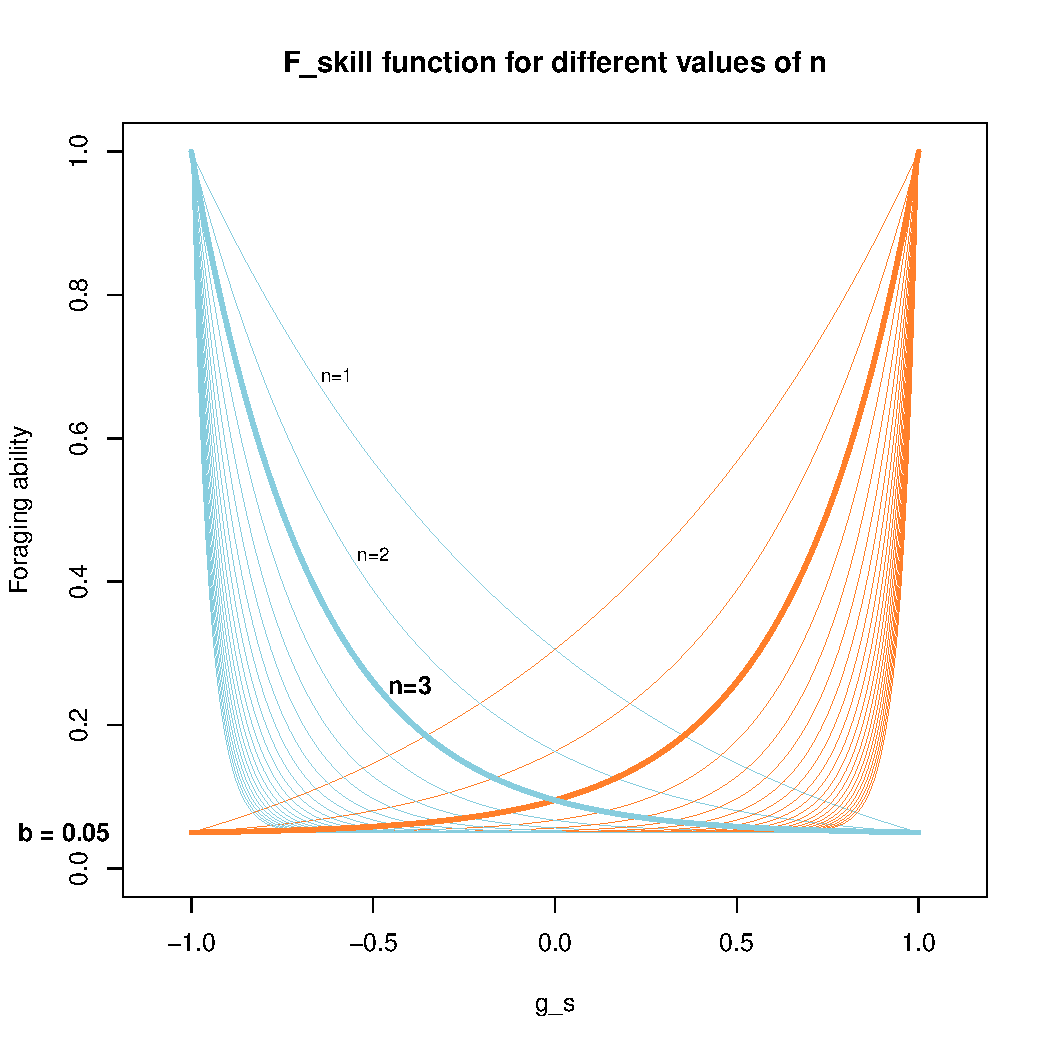
\includegraphics[height=6cm]{images/f_skill_alpha}
\end{figure}


	\column{0.50\textwidth}
 $$ f_{skill}(g_{s,i},type_Q)= {\frac{\left(e^{n*g_{s,i}*t_q}\right)+C(b,n)} {e^{n}+C(b,n)}}$$
\begin{enumerate}
	\item[ $\rightarrow$] Tune $f_{skill}$ : $n=?$, $b=?$
% 	\item Fix $\alpha$ to force specialization.
\end{enumerate}

\end{columns}


\end{frame}

%%%----------------------------------------------------------------------
%%%----------------------------------------------------------------------
\begin{frame}{Some first results}
\begin{figure}
 \includegraphics[height=7cm]{images/0523_08h28}
						%the heatmap for exemple, and one rune, why not a beautiful tree with beautiful speciation
\end{figure}

\end{frame}

%%%----------------------------------------------------------------------
%%%----------------------------------------------------------------------


\begin{frame}{Next steps}
\begin{itemize}
 \item resources limitations
 $$F_{rwd,t}(i,Q) = f_{skill}\left(g_{s,i},T_Q\right)\times d_{penality}\left(h_{Q,t}\right)\times \alpha$$
 \item specialists vs. generalists
 \item from specialization to (sympatric?) speciation
%  \item changing environment: switch between one and two types, variate environmental setting \emph{during} the run,...
 %\item n type off resources
\end{itemize}

\end{frame}


%%%----------------------------------------------------------------------
%%%----------------------------------------------------------------------

%\begin{frame}{Short biblio}
% 
%\begin{columns}
% 

% 
%\column{0.75\textwidth}
%	\small
% \bibliographystyle{plainnat}
% \bibliography{/home/simon/evorob/Doc/bib/simon.bib}
%%  
% \end{columns}
% 
% 
%\end{frame}
% 
 \begin{frame}%\addtocounter{framenumber}{-1}
 \begin{center}
  Thank you for your attention.
  \end{center}
 \end{frame}

 %%%----------------------------------------------------------------------
 %%%----------------------------------------------------------------------
 
 %%%----------------------------------------------------------------------
 %%%----------------------------------------------------------------------
 
\begin{frame}{Add a density pressure}\addtocounter{framenumber}{-1}

$$F_{rwd,t}(i,Q) = f_{skill}\left(g_{s,i},T_Q\right)\times d_{penality}\left(h_{Q,t}\right)\times \alpha$$

\begin{columns}

\column{0.50\textwidth}


 	\begin{itemize}
 		\item $i$ the agent,
 		\item $t$ the iteration of the simulation,
 		\item $ d_{penality}(h_{Q,t}) =  1 - \frac {h_{Q,t}} {nrobots} $
 		\item $ f_{skill}(g_{s,i},type_Q)= {\left(e^{n*g_{s,i}*t_q}\right)+C(b,n) \over {e^{n}+C(b,n)}}$
 		\item $h_{Q,t} \in [0, n -1]$ the number of robot harvesting $Q$ at $t$ 
 		\item $g_{s,i} \in [-1,1]$ the value of the gene for the foraging skill of $i$,
 		\item $T_Q\in \{-1,1\}$ the type of the resource Q
 		\item $ C(b,n) = {(be^{n} - e^{-n} )\over{(1-b)}} $
 	\end{itemize}


% where  , $n$ and $C(b)$ are two parameters allowing us to tunes the environment hostility.





\column{0.50\textwidth}

\begin{figure}
\includegraphics[height=6cm]{images/densite}
\end{figure}


\end{columns}


\end{frame}


\end{document}
